\subsubsection{Moving average filter}
Moving average filteret testes for at undersøge hvorvidt de opstillede krav beskrevet i \autoref{fig:mavg_test} overholdes, samt undersøge om designet er korrekt implementeret. Måden hvorpå dette testes er ved anvendelse af data fra pilotforsøget, da dette giver kontrolleret testforhold. 
En computer med MATLAB benyttes til at sende en givene måling til mikrokontrolleren hvorpå filteret er implementeret. Mikrokontrolleren returnere løbende den filtrerede værdi, der visualiseres i MATLAB. Udfra dette ses om filteteret virker hensigtsmæssigt. 

Resultatet af dette test fremgår af \autoref{fig:mavg_test}. 

\begin{figure}[H]
	\centering
	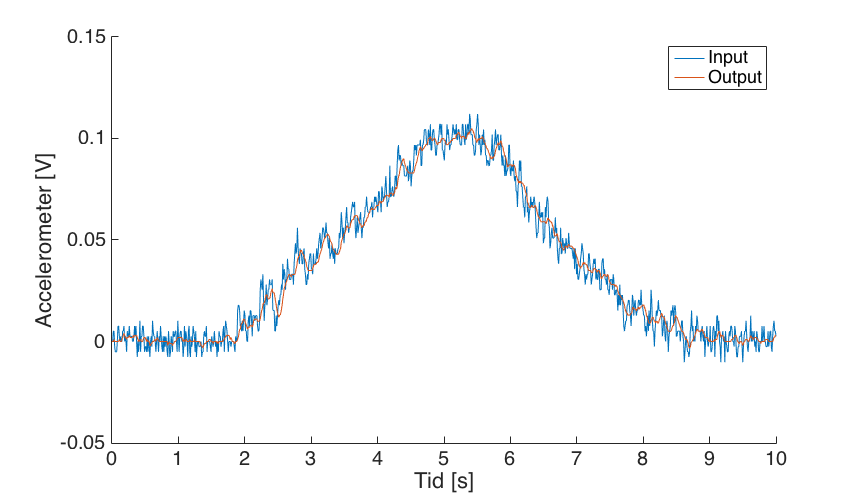
\includegraphics[width=1\textwidth]{figures/accelerometer_filter}
	\caption{Moving average filter test, visualiseret i MATLAB}
	\label{fig:mavg_test}
\end{figure}

\noindent
Da filteret kræver 10 samples for at retunere den første værdi testes det, hvorvidt dette stemmer overens med det forventede forsinkelse på $100~ms$. 

Resultatet fra denne test.... %% Dette vil jeg gerne sprøge steffen om i morgen, altså om hvordan jeg videnskabeligt kan beregne eller aflæse den forskydelse som kan ses af grafen. 

Yderligere foretages en test af forsinkelsen der forekommer i det filteret eksekveres. Til denne test er en debug pin blevet defineret, hvor denne pin sættes som høj før funktionskaldet, og lav efter funktionskaldet. Et oscilloscope tilsluttes debug pin, således det kan måles hvor længe debug er høj. Af dette kan en forsinkelse aflæses af oscilloscopet. 
Resultatet fra testen er en forsinkelse på $320~\mu s$, for data at passere filteret. Dette betragtes som værende ikke af signifikant betydning.    
Ud fra ovenstående resultater vurderes det, at det filterede signal opfylder kravene for \autoref{sec:mavg_krav}. 